\title{Arjun Trivedi's contribution to the NIM publication}
\date{June 05, 2014}

\documentclass[12pt]{article}

\usepackage{hyperref}
\usepackage{cite}

\usepackage{graphicx}
%\usepackage{epsfig}
\usepackage{epstopdf}

\usepackage{mathtools}
\newcommand{\defeq}{\vcentcolon=}

\usepackage{float}
\restylefloat{table}

\begin{document}
\maketitle

% \begin{abstract}
% This is the paper's abstract \ldots
% \end{abstract}

\section{III.E. Photomultiplier tubes (PMTs)}

\subsection{Different PMTs time resolutions}
\textit{My assumptions in writing this section}
\begin{enumerate}
	\item \textit{Our chosen PMT(R9779) was compared with panel-1a PMT(EMI9954A)}
	\item \textit {Details of relevant differences of the tech-specs of the two PMTs and therefore the expected superiority of R9779 over EMI9954A will be listed elsewhere; here we will only give empirical proof}
\end{enumerate}

\textit{By the way, can we use the web link directly to Felician's page as a reference? Perhaps not, but this is just to make a note to confirm this.}

The selected Hamamatusu's R9779 PMTs for panel-1b were compared with Electron Tubes EMI 9954A in the 3-bar setup (\textit{I am assuming that the 3-bar setup will either already be defined or referred to in another publication, so as to not go into details, but simply for the reader to trust that it is our way to extract time-resolution, though, it is NOT directly the time-resolution of the PMT, but of the entire counter; this is important to keep in mind, since for the old TOF system, PMT resolutions were directly compared using lasers; details of this method are in old CLAS-SC NIM paper.})

\textit{Should I mention here that for EMI PMT tests, the contribution of the LFIO module was removed?}

\newpage
Below is the figure that shows the superiority of the R9779:
\begin{figure}[th]
	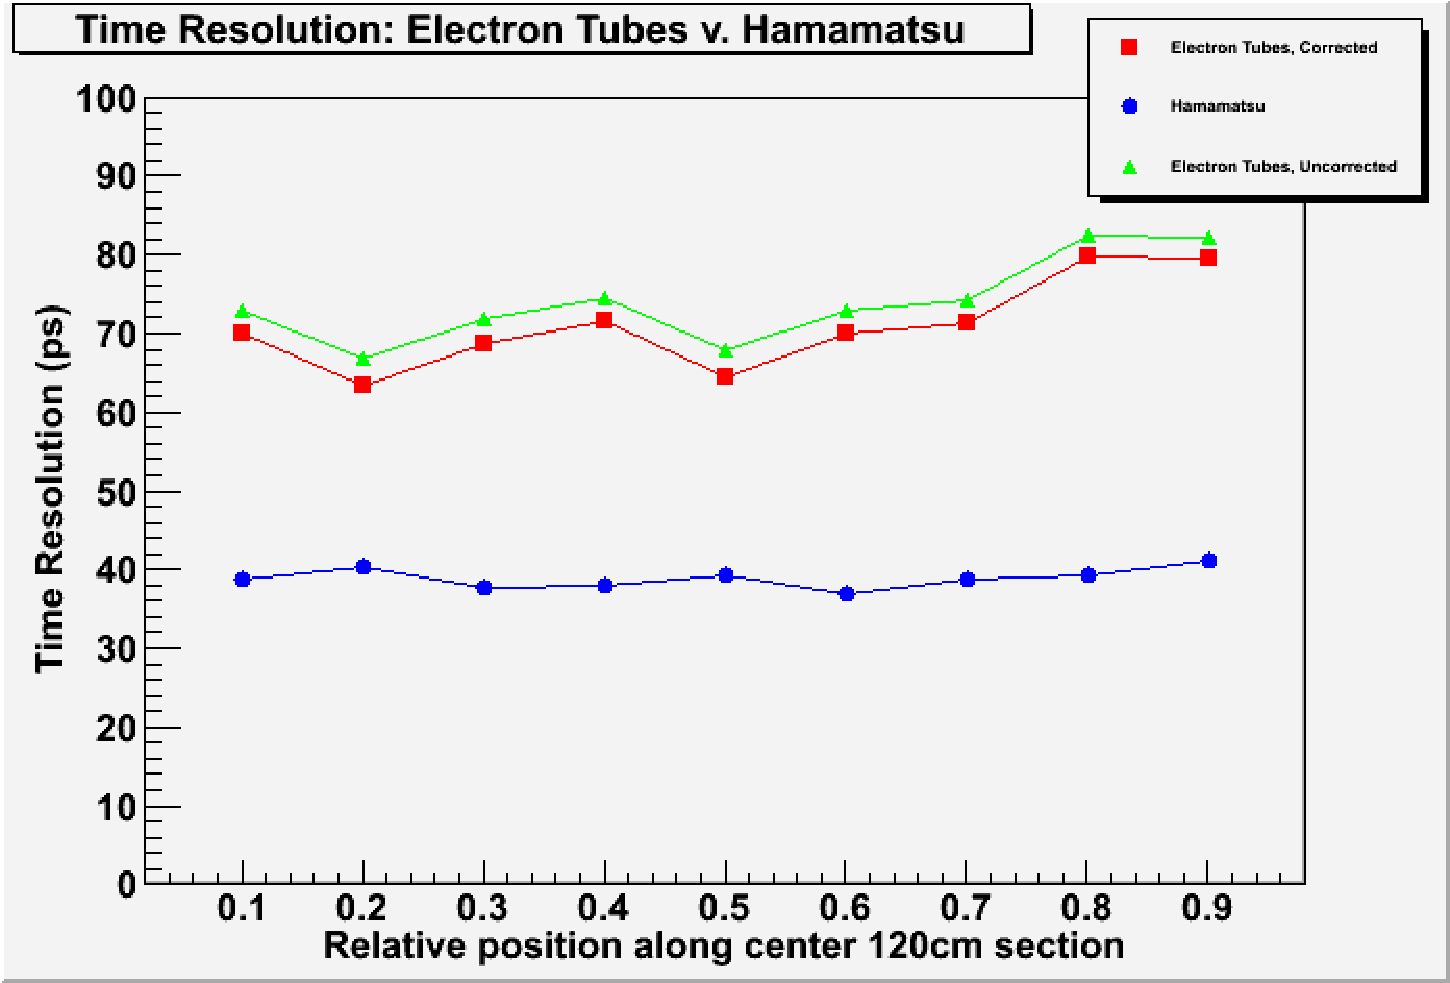
\includegraphics[width=10cm, height=5cm]{PMTcomparison.pdf}
\end{figure}

\subsection{... threshold dependence}
\textit{This section is still lazily written}
We also compared various threshold (\textit{Define "threshold"}) levels for the signals from the PMT and see if it had any affect on the time resolution. The threshold levels tried were:50mV, 75mV, 150mV, 300mV, and 600mV.

Following is a figure that demonstrates varying the threshold did not affect the time resolution.
\begin{figure}[th]
	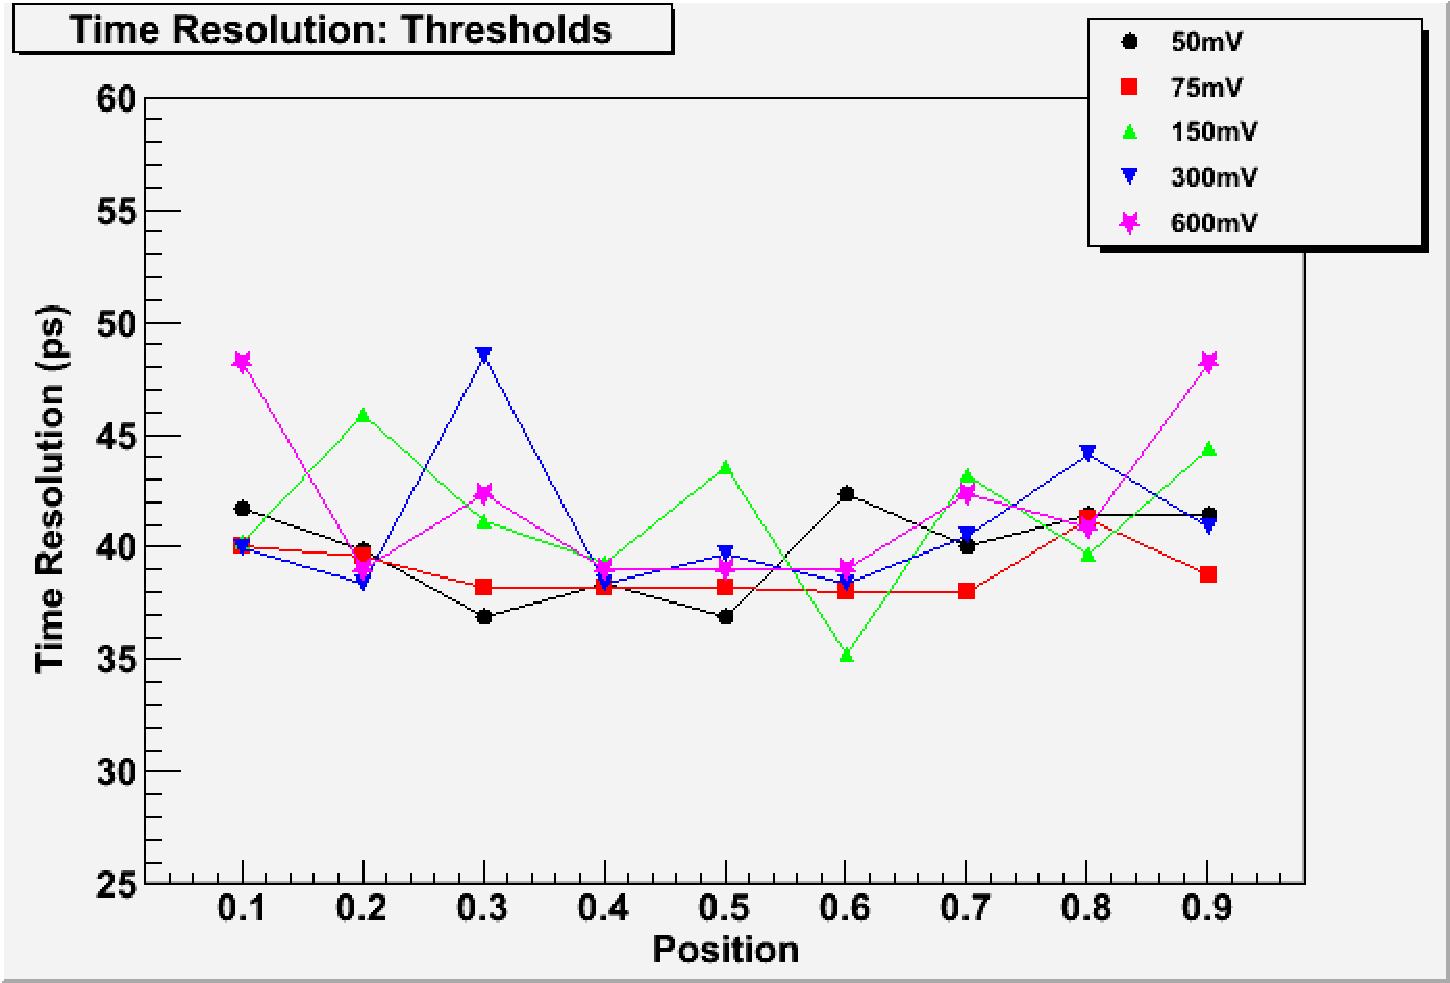
\includegraphics[width=10cm, height=5cm]{ThresholdsTimeRes.pdf}
\end{figure}

\section{III.G. Magnetic shielding of the PMTs}
The photomultipliers that are attached to the FTOF scintillators will be exposed to the combined stray magnetic fields from the CLAS12 solenoid and torus magnets. It is therefore important to study the effect of the magnetic field strength on the anode signal of a PMT and ultimately on the time resolution of the FTOF detector system. In the experimental test setup, a PMT was set on a flat, non-magnetic base in between a Helmholtz coil and the anode signal of the PMT was read by a DAQ system (\textit{I think there is no need for a detailed write and diagram up on the DAQ for it is essentially that same as that of the 6-bar procedure, which will already be described in detail}). This arrangement is shown in Fig. XX.

\textit{Illustration figure: xfig or photograph as used by RS}

Due to the dynode-array geometry of the PMT and the electrodynamic processes which finally contribute to the signal formation, the studies need to be performed under particular orientations of the PMT relative to the magnetic field. Given the axial Helmholtz magnetic field, the orientation of a PMT in it can be described by two rotational degree of freedoms; their axes are illustrated in Fig. XX and defined by the PMT's axis of cylindrical symmetry, $\hat{z}$ and the radial axis perpendicular to $\hat{z}$ and horizontal to the flat base supporting the PMT, $\hat{\rho}$.

\textit{Illustration figure: xfig}

In the axial Helmholtz magnetic field, a PMT can be rotated around $\hat{\rho}$ until $\hat{z}$ is aligned transversely (T) or longitudinally (L) with the field direction. These are the two orientations in which a PMT is observed to have the two strongest and in a sense, independent responses; any other orientation is dominated by a superposition of the two responses. 

The additional change in the signal response of a PMT when it was rotated around $\hat{z}$ was also studied, primarily when it is already aligned in the transverse orientation (minimal to no effect due to rotations around $\hat{z}$ is expected in the longitudinal orientation) \cite{Steinman} (\textbf{Re-do measurements:} Steinman has data for rotations around $\hat{z}$ in the transverse orientation; the fact that there will be minimal impact in the longitudinal orientation is what I am hypothesizing). However, after implementing the final shielding configuration (see Fig. XX), the PMT response no longer depends on the rotational degree of freedom around $\hat{z}$.

It is worth mentioning here that the magnetic field primarily affects the signal amplitude, while the signal shape and smoothness, which have a far larger impact on the time resolution, are mostly unaffected \cite{Steinman}. However, the loss of signal amplitude, does affect the extracted time resolution, but only when the reduction is significant. Therefore, the signal amplitude was used as the parameter to quantify the response of a PMT in a magnetic field and its affect on the time resolution. Even though it was established that when the signal amplitude is reduced by 10\%(\textbf{Measurement of reduction at 10G-L or at which XX-L is reduction = 10\%}) in the longitudinal and X\%(\textbf{Measurement of reduction at 20G-T}) in the transverse orientations there is no change in the time resolution \cite{Steinman}, the final design of the magnetic shielding is such that up to magnetic field strengths higher than those expected in CLAS12, the PMT signal amplitude shows no reduction (\textit{I feel like we need to justify this "conservative" approach. I have laid out my finding on this matter based on historical research in the section: Test results and the final design of the magnetic shielding}). (The maximum (\textit{anticipated?}) stray field strength that the panel-1b PMTs are going to be exposed to is expected to be 22G, of which 2/3 (15G) will be in the axial direction (\textit{Mention where exactly in CLAS12 this maximum will be present}) \cite{CLAS12FTOFstudies} and the tests at USC were done with magnetic fields up to 25G, wholly directed in either the transverse or longitudinal directions.(\textit{actually 30G, but my hesitation in stating so, will be reflected later}))

\subsection{Initial design considerations}
The PMTs were already manufactured with a layer of mu-metal coating (\textit{Do we need to be precise here about the thickness of the coating and/or any other important details?}). It can be seen from the following table that in the transverse orientation, compared to a PMT without any mu-metal coating, the inbuilt mu-metal shielding preserved the signal amplitude to much higher levels of magnetic fields.

% \begin{tabular}{|r|l|}
%   \hline
%   7C0 & hexadecimal \\
%   3700 & octal \\ \cline{2-2}
%   11111000000 & binary \\
%   \hline \hline
%   1984 & decimal \\
%   \hline
% \end{tabular}

\begin{table}[H]
	\begin{center}
		\begin{tabular}{|c|c|l|}
			\hline
	 		& no mu-metal & with mu-metal \\
			\hline
 			10G-L & 10\% & 10\% \\
 			10G-T & 100\% & 0\% \\ 
 			\hline
 			15G-L & XX\% & XX\% \\
 			15G-T & 100\% & 0\% \\
 			\hline
 			15G-L & YY\% & YY\% \\
 			15G-T & 100\% & 0\% \\
 			\hline
 			20G-L & ZZ\% & ZZ\% \\
 			20G-T & 100\% & 10\% \\
 			\hline
 			25G-L & AA\% & AA\% \\
 			25G-T & 100\% & XX\% \\
 			\hline
 			30G-L & BB\% & BB\% \\
 			30G-T & 100\% & BB\% \\
 			\hline
		\end{tabular}
	\end{center}
	\caption{Reduction of PMT anode signal in various test configurations}
\end{table}


Even with the inbuilt mu-metal shielding, there is a rapid deterioration of the signal past 10G-L and XXG-T and this led to considering further shielding methods.

\subsubsection{External shielding}
\textit{Historical interlude to reconstruct the "initial design considerations" for external shielding and "final implementation of shielding with overhang". I want to faithfully reproduce the considerations that led to the "final shielding design and implementation". This was prompted by my own need to justify certain design considerations and if the answers I arrived at were indeed correct, for example:
\begin{itemize}
	\item Why did we use $25\;G(30\;G?)$ as the upper limit for preserving signal amplitude?\\
	\newline
	Because to me it appears that at the time of the initial design of the shielding, the upper limit of the magnetic fields in CLAS12 was not established. We decided to shield the PMTs "from higher than expected magnetic fields" in CLAS12 and $25\;G(30\;G?)$ - the capacity of Helmholtz coils at USC - incidentally happened to match the critereon. \\
	\newline
	Incidentally (or was it more than that?), it turns out that protecting the PMT signal in the longitudinal direction up to $25\;G$ fits in with the general shielding design philsophy of panel-1a($2\;in$ PMTs) and panel 2($3\;in$ PMTs); the maximum fields to which their PMTs will be exposed to are $17\;G$ and $28\;G$ respectively (of which roughly 2/3 will be in the axial direction) and their designed shielding offers protection to up to $20\;G$ and $30\;G$ respectively \cite{CLAS12FTOFstudies}. In that sense, panel-1b PMTs will be exposed to a maximum field of $22\;G$ (of which 2/3 will be in the axial direction) \cite{CLAS12FTOFstudies} and therefore, the upper limit of $25\;G(30\;G?)$ we settled on is consistent with the general shielding philosophy.\\
	\item Why the rectangular geometry?\\
	\newline
	This is directly stated, but to me appears to based on an ansatz that was empirically proven to be effective.(It may have been motivated by the rectangular geometry of the scinitallator bar on its backing structure)
\end{itemize}
}
\begin{itemize}
	\item \textbf{Consideration:} To preserve signal integrity up to $25\;G(30\;G?)$ in the transverse and longitudinal orientations
	\item \textbf{Final design and implementation:} External mu-metal shielding, each side of width $2\;mm$, enclosing the PMT to a depth of $4\;cm(1.5\;in)$
\end{itemize} 

In the research that follows, I will quote directly from the following sources used for historical research(if not stated otherwise):
\begin{enumerate}
	\item Rob Steinman's thesis
	%\item Anecdotal sources for "final implementation of shielding with overhang" 
\end{enumerate} 

\textbf{Adopting $25\;G(30\;G?)$ as the upper limit} \\
It seems that initially, the upper limit of the magnetic field at Jlab was not known; therefore, at USC we decided to decided to shield the PMTs "from higher than expected magnetic fields":\\
\newline
"The strength of the magnetic field at Jefferson Lab has yet to be determined, though it will supposedly be below 20 G. While awaiting the final values, the University of South Carolina has been exploring alternative methods for shielding the PMTs from higher than expected magnetic fields."\\
\newline
I will assume for the time being that since at USC fields up to $30\;G$ could be produced, we used that as our upper limit in the design consideration.\\
\newline
\textbf{Further shielding considerations} \\
"Two options can further shield the PMTs from magnetic fields": External mu-metal shielding and Active shielding \\
\newline
%\paragraph{External mu-metal shielding}
\textbf{External mu-metal shielding} \\
\newline
\textbf{Rectangular geometry} \\
The following lines seem to justify the rectangular geometry for the shielding:\\
\newline
"The construction designs for the FTOF detector at Jefferson National Lab allows for additional mu-metal shielding for the PMTs if the magnetic field intensity proves larger than expected. Many different configurations of shielding can be used, though the current design decision is based on a rectangular box which will cover the PMT to the actual scintillator."\\
\newline
The decision to use a rectangular design is directly stated. It may be nice to mention if this decision was based on ansatz, wich in turn was motivated by the rectangular configuration of the scintillar and the backing structure?\\
\newline
\textbf{Note for internal discussion of the fact that initially it was considered important to not cover the scintillars with mu-metal shielding} \\
I am stating the following just to make a point to discuss that finally we did shave the edges of the bars to shield from longitudnal fields, even though initially it was considered "important" to not cover the scintillator with mu-metal shielding\\
\newline
"It is important not to cover the scintillator with mu metal because the counters are stacked and would require trimming to fit the additional shielding." \\
\newline
\textbf{Rectangular geometry: thickness of edges} \\
The following states the initial widths of the sides of the external shielding used for testing:\\
\newline
"The width of the box used in the experiment can be adjusted by adding additional mu-metal plating along the four sides and the end piece encapsulating the PMT as needed by the design. Figure 19 shows the shielding design schematic and, for the purposes of this experiment, the sides are 2 mm thick, while the end piece is 5 mm."
\newline

The following states the results of the test, whereby it was seen that the signal is preserved up to 25G-T with the external shielding, with no benefits of shielding from longitudnal fields (the additional width of $5\;mm$ at the ends made no difference):\\
\newline
"The magnetic field is adjusted to 25 G to once again analyze the effects of large transverse fields. The ADC distribution shows that the signal has been preserved even under transverse fields with the additional mu-metal shielding surrounding the PMT. The axial fields, however, are not shielded by this mu-metal shield. This, again, makes sense, because the axial fields are incident on the photocathode, where there is no shielding. It was hoped that the thick end plate on the mu-metal box would help to shield against the axial fields, but this was not the case."\\
\newline
\textbf{My conclusion} \\
Therefore, I conclude that initially, an external mu-metal shielding was one of the ways considered to shield the PMT. Since the upper limit of the magnetic fields in CLAS12 was unknown at the time, we designed an external mu-metal shielding (rectangular; each side of width $2\;mm$) that would preserve the signal from transverse fields up to maximal fields we could reach at USC i.e. $25\;G(30\;G?)$ (which incidentally(?) happened to coincide with the general philosophy of shielding design for FTOF PMTs in CLAS). It was observed that the desgigned external shielding would not provide any additional protection to the PMT signal from longitudinal fields. 

The following table will need to be filled out to support the statements.

\begin{table}[H]
	\begin{center}
		\begin{tabular}{|c|c|}
			\hline
	 		& external mu-metal shielding \\
			\hline
 			10G-L & 10\% \\
 			10G-T & 0\% \\ 
 			\hline
 			15G-L & XX\% \\
 			15G-T & 0\% \\
 			\hline
 			15G-L & YY\% \\
 			15G-T & 0\% \\
 			\hline
 			20G-L & ZZ\% \\
 			20G-T & 0\% \\
 			\hline
 			25G-L & AA\% \\
 			25G-T & 0\% \\
 			\hline
 			30G-L & BB\% \\
 			30G-T & BB\% \\
 			\hline
		\end{tabular}
	\end{center}
	\caption{Signal reduction of PMT's anode signal in presence of external mu-metal shielding. It is observed that PMT signal's reduction is unchanged in the longitudinal orientation, but the signal is preserved to $25\;G(30\;G?)$ in the transverse orientation}
\end{table}
\newpage

%\paragraph{Active shielding}
\textbf{Active shielding (Mentioned for the sake of integrity of historical research)} \\
Following is note on the considered active shielding for the PMTs:\\
\newline
"There are further options for shielding the PMTs from axial fields. One option is to apply active shielding to the PMT by wrapping it in a coil and running a current through. This will create a magnetic field which should counteract the axial fields inside the FTOF detector. Without knowing the exact magnetic field values, however, no final decisions can be made at this time. The group in charge of the magnetic field calculations at Jefferson Lab must supply the University of South Carolina with the final estimate values in order to finalize the  construction process of the PMTs as well as the need for additional shielding on site."
\newline
This additionally confirms to me that when the shielding was initially being designed, the maximum field levels in CLAS12 were not known. Otherwise, steps would have been taken to shield the PMT from the more challenging, longitudinal fields.

\subsection{Final implementation of shielding with overhang}
To preserve the signal amplitude in the longitudinal orientation, it was decided that in the final implementation, the external shielding would extend a few inches ($\defeq$ overhang) beyond the front face of the PMT (This was would require shaving the edges of the scintillator bars). The following table shows the results of testing the signal reduction at various overhang positions of the external shielding. The overhang position of $1.5\;in(4\;cm)$ is sufficient to preserve the signal up to $25\;G$ in the longitudinal orientation.

\begin{table}[H]
	\begin{center}
		\begin{tabular}{|c|c|c|c|c|c|}
			\hline
	 		& $0\;cm$-overhang & $1\;cm$-overhang & $2\;cm$-overhang & $3\;cm$-overhang & $4\;cm$-overhang \\
			\hline
 			10G-L & & & & & \\
 			10G-T & & & & & \\ 
 			\hline
 			15G-L & & & & & \\
 			15G-T & & & & & \\
 			\hline
 			15G-L & & & & & \\
 			15G-T & & & & & \\
 			\hline
 			20G-L & & & & & \\
 			20G-T & & & & & \\
 			\hline
 			25G-L & & & & & \\
 			25G-T & & & & &\\
 			\hline
 			30G-L & & & & & \\
 			30G-T & & & & & \\
 			\hline
		\end{tabular}
	\end{center}
	\caption{Signal reduction of PMT's anode signal in presence of external mu-metal shielding at various overhang positions. It is observed that at overhang position of $4\;cm$ the signal is preserved up to magnetic field strength of $25\;G$ in both the transverse and longitudinal orientations}
\end{table}


\section{Establishing an upper limit on levels of magnetic field tolerance}
In the final design and implementation of the magnetic shielding, the tests show that there is going to be no reduction in signal amplitude in fields up to $25\;G$ in the transverse and longitudinal orientation. This is already beyond the maximum fields to which the PMTs will be exposed to in CLAS12. However, we did run tests, to note signal reduction factors as we increased the magnetic field beyong $25\;G$ in each of the orientations and noted the point at which the signal amplitude reduced by 10\% and X\% in the longitudinal and transverse orientations respectively. Since we know that up to such reduction factors, the time resolution is unaffected, the noted field strength would serve as the minimum upper limit of the magnetic field at which the time resolution is unaffected. The following table shows the results of such tests which establishes the minimum upper limit at which the time resolution is unaffected at $XX\;G$ and $YY\;G$ in the transverse and longitudinal orientations respectively.

\begin{table}[H]
	\begin{center}
		\begin{tabular}{|c|c|}
			\hline
			30G-L &  \\
 			30G-T &  \\ 
 			\hline
 			35G-L &  \\
 			35G-T &  \\
 			\hline
 			40G-L &  \\
 			40G-T &  \\
 			\hline
 			45G-L & \\
 			45G-T &  \\
 			\hline
 			50G-L &  \\
 			50G-T &  \\
 			\hline
 		\end{tabular}
	\end{center}
	\caption{Signal reduction of PMT's anode signal beyond the design consideration of $25\;G$}
\end{table}


\subsection{Results and Conclusions}
With the finally designed and implemented shielding, the time resolution from the panel-1b FTOF counters is unaffected due to presence the magnetic fields in CLAS12 to up to field levels of $XX\;G$ and $YY\;G$ in the transverse and longitudinal orientations respectively. This exceeds the maximum fields to which the panel-1b PMTs are expected to be exposed to ($22\;G$ of which 2/3 will be in longitudinal direction). 



% \phantomsection
% \addcontentsline{toc}{chapter}{Bibliography}
\label{bib}
\bibliographystyle{abbrv}
\bibliography{at_contrib}

\end{document}